\section{Magnetic Resonance Imaging~(MRI)}

\begin{frame}[plain,c]
    %\frametitle{A first slide}
    
    \begin{center}
        \color{DarkBlue}
    \Huge \insertsection
    \end{center}
    
\end{frame}

\begin{frame}{What does an MRI look like?}
    \begin{figure}
        \centering
        \begin{subfigure}{0.45\textwidth}
            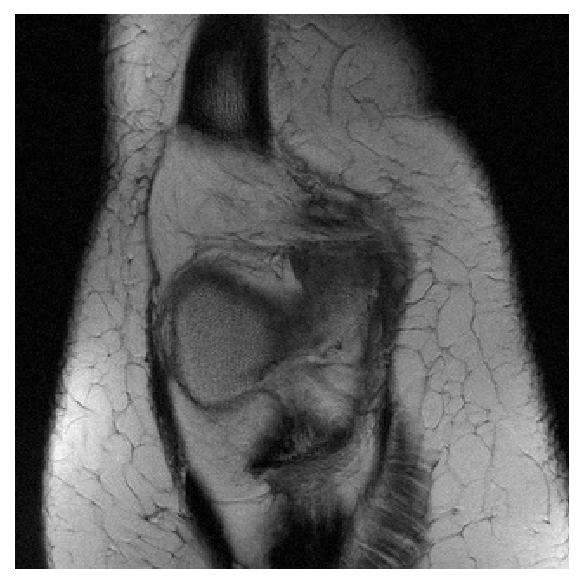
\includegraphics[height=0.6\textheight]{Figures/intro_figures/example_knee_fastmri.pdf}
        \end{subfigure}
        \begin{subfigure}{0.45\textwidth}
            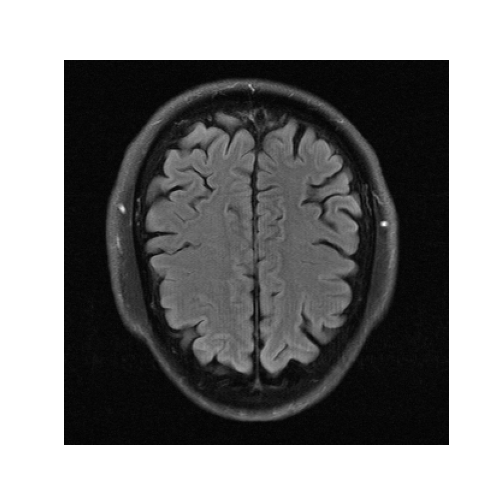
\includegraphics[height=0.6\textheight]{Figures/intro_figures/brain_mri.png}  
        \end{subfigure}
        \caption{\label{fig:mri-example} \textbf{Examples of MR images}: knee and brain taken from the fastMRI dataset.\footfullcite{Zbontar}}
    \end{figure}
    % explain content of image: it's not a photo, but it tells us the tissue density
    % explain that MRI is non invasive an high res!
\end{frame}



% MRI is so popular why isnt it solved already ?
\begin{frame}{Physics of MRI: Nuclear Magnetic Resonance and k-space}
    \begin{center}
        \begin{tikzpicture}[
            >=stealth,font=\Large, node distance=0.5em,
            b0/.style={line width=7pt, draw=DarkGreen},
            spin/.style={line width=2pt},
            excit/.style={line width=8pt},
            pulse/.style={line width=3pt, color=amber!87},
            pulse_text/.style={above,midway,color=amber!87},
        ]
        % nodes
        \node[] (mri) at (-7cm, 1cm) {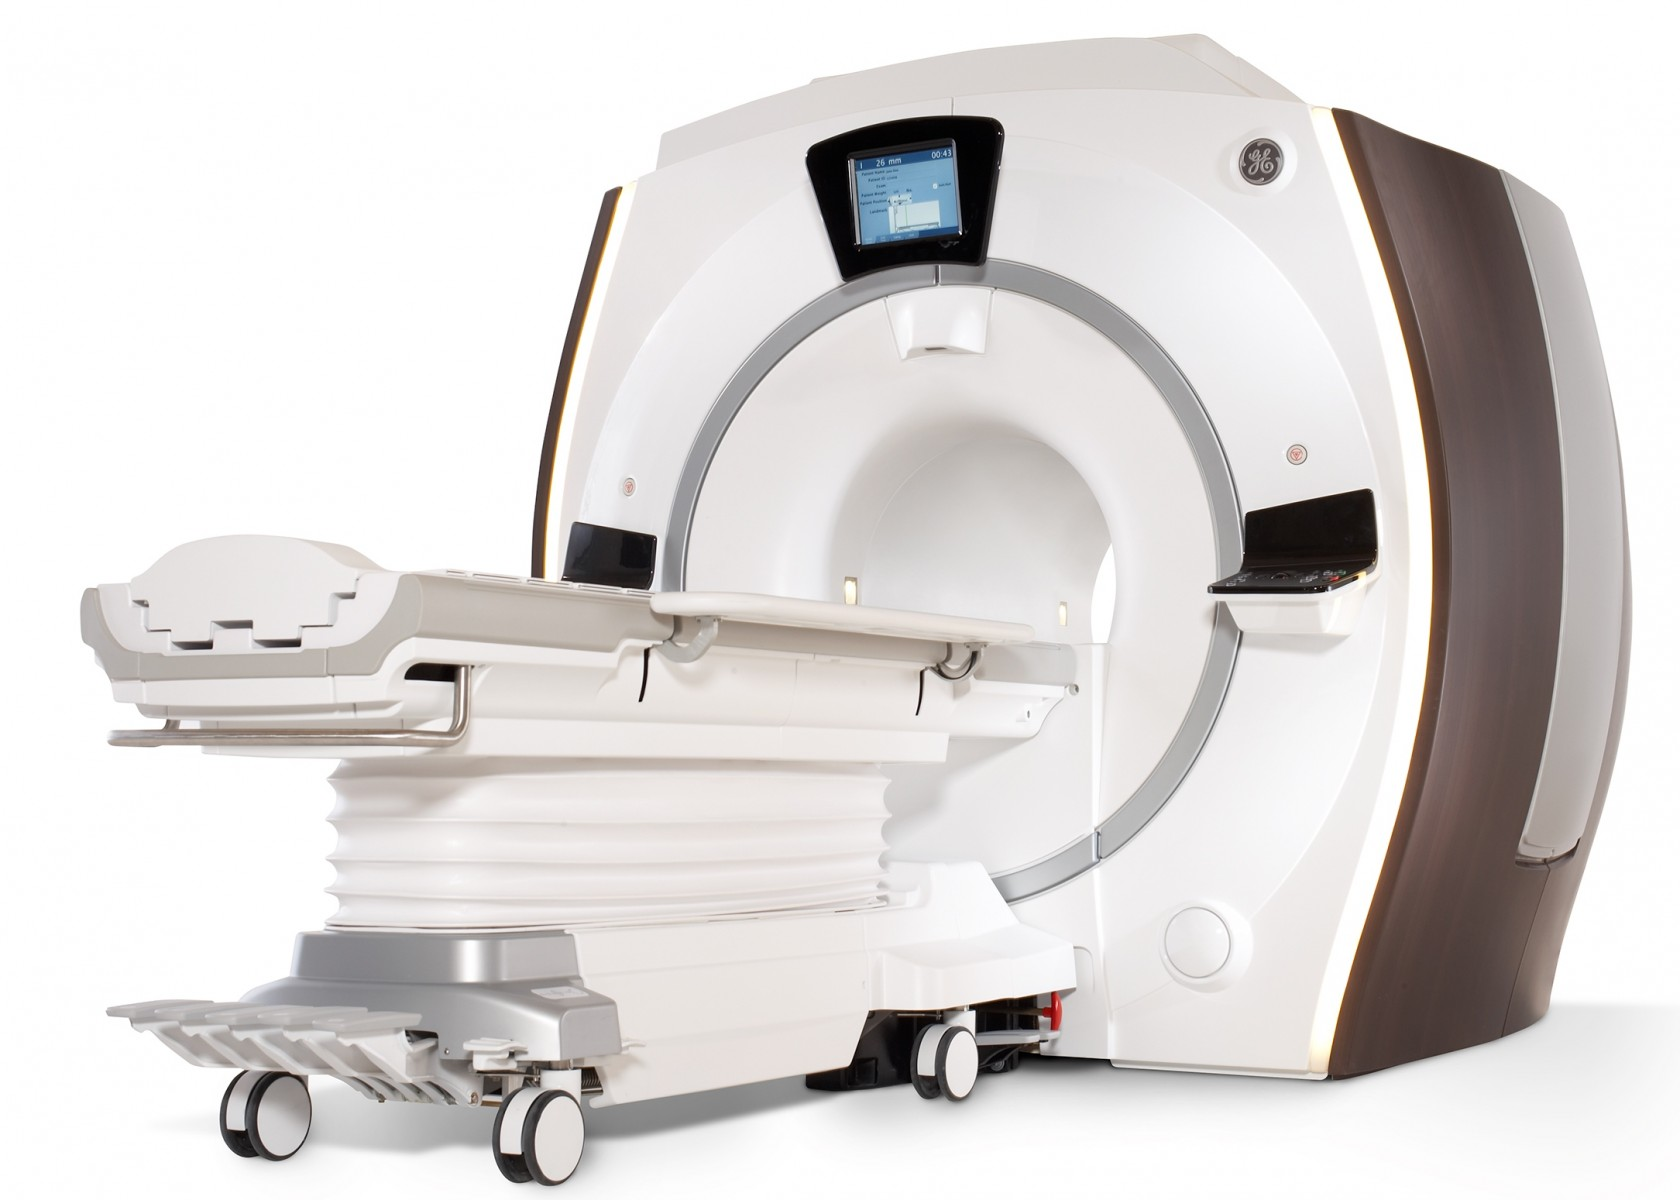
\includegraphics[height=0.3\textheight,]{Figures/intro_figures/mri.jpg}};
        \node[below=of mri] (brain) {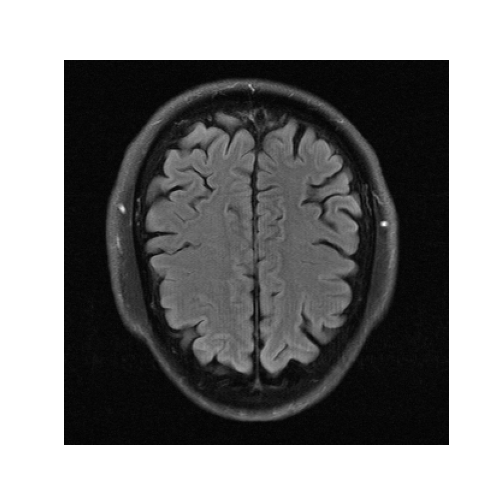
\includegraphics[height=0.3\textheight,angle=180]{Figures/intro_figures/brain_mri.png}};
        \shade[ball color = blue!47] (0,0) circle (1cm);
        \node(coil) [circle, draw, visible on=<3->] at (4.5cm,0) {\textbf{Antenna}};
        \node[visible on=<2->] (bottom_arrow) at (0, -1.8cm) {$\Bb_0$};
        \node(kspace) [visible on=<4->, below=of coil] {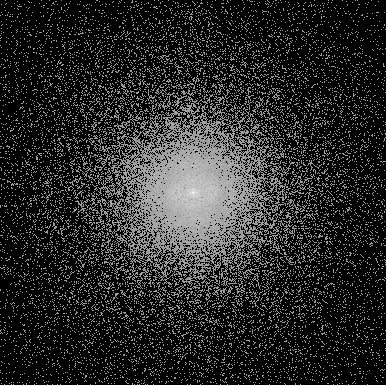
\includegraphics[width=0.13\textwidth]{Figures/intro_figures/kspace_phantom.png}}; 
        %% excitation / relaxation
        \draw[excit, visible on=<2>, color=red!87,->] (-1.3cm,1.6cm) arc [start angle=95, end angle=175, x radius=1.6cm, y radius=1.6cm] ;
        \node [color=red!87, visible on=<2>] at (0, 2cm) {\textbf{Excitation}};
        \draw[excit, visible on=<3->, color=green!87, <-] (-1.3cm,1.6cm) arc [start angle=95, end angle=175, x radius=1.6cm, y radius=1.6cm];
        \node(arrow_relax_end) at (-2.8cm, 0) {};
        \node(text_relax) [color=DarkGreen!87, visible on=<3->] at (0,2cm) {\textbf{Relaxation}};
        \node(fit_relax) [visible on=<5->, fit=(text_relax) (bottom_arrow) (arrow_relax_end), draw=red!47, dashed] {};
        \node(text_slow) [visible on=<5->, above right=-1.3em and 0 of fit_relax, color=red!47] {\textbf{This is slow!}};
        %% pulses
        \draw[<-, pulse,visible on=<2>] (1.9cm,0cm) -- node [pulse_text] {\textbf{RF pulse}} ($(coil.west)+(-0.3cm,0)$);
        \draw[->, pulse,visible on=<3->] (1.9cm,0cm) -- node [pulse_text] {\textbf{FID}} ($(coil.west)+(-0.3cm,0)$);
        %% arrow spin
        \draw<1,3>[->,spin] (-0.3cm,0.8cm) -- (-0.6cm,1.6cm);
        \draw<2>[->,spin] (-0.9cm,0.cm) -- (-1.8cm,0cm);
        \begin{scope}[on background layer]
            \draw<1,3>[spin] (0.3cm,-0.8cm) -- (0.6cm,-1.6cm);
            \draw<2>[spin] (0.9cm,0cm) -- (1.8cm,0cm);
            %% field
            \draw[->,-{Triangle[width=18pt,length=9pt]}, b0]  (0, -1.5cm) -- (0, 1.75cm);
        \end{scope}
        % arrows
        \draw[->, visible on=<1>] (mri.east) --  (-0.2cm, -1.4cm);
        \draw[->, visible on=<1>] (brain.east) --  (-0.71cm,-0.71cm);
        %% spin
        \begin{scope}[on background layer]
            \draw<1>[->,dashed,semithick] (-0.6cm,1.6cm) arc [start angle=180, end angle=-70, x radius=0.6cm, y radius=.1cm];                
        \end{scope}
        %% signal recording
        \draw[->, visible on=<4->] (coil.south) -- ($(kspace.north)+(0,-0.1cm)$);
        %% ift
        \draw[->, line width=0.3cm, color=DarkBlue, visible on=<4->] (kspace.west) -- ($(brain.east)+(-0.3cm,-0.5cm)$) node [below,midway, color=DarkBlue!87, yshift=-0.3cm] {\textbf{IFFT}};
            
        \end{tikzpicture}
    \end{center}
    
\end{frame}



\begin{frame}{Physics of MRI}
    % Let's not forget our initial goal here: we want to understand why MRI is slow
    % The relaxation is slow !
    \begin{block}{Recap}
        MRI relies on the nuclear magnetic resonance phenomenon. This enables us to sample the Fourier space of the anatomical object of interest.
        MRI is slow, because the \textbf{relaxation} is slow!
    \end{block}
    \pause
\end{frame}

\begin{frame}{Acceleration}
    % Explain the concept of redundancy
    % first example: partial Fourier $\Rightarrow$ give limits
    % \textbf{Redundancy}, otherwise called \textbf{sparsity, symmetry, structure or a priori information}, is the core concept that will help us accelerate MRI.\\
    Naively: sample fewer lines in the k-space.
    \vspace{-2em}
    \begin{center}
        \begin{tikzpicture}[>=stealth]
            \node (kspace) {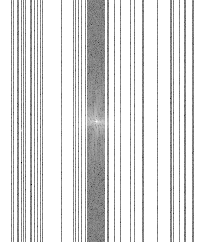
\includegraphics[width=0.25\textwidth]{Figures/intro_figures/kspace_mri.png}};
            \node[below=0.7em of kspace] (kspace_exp) {Undersampled k-space};
            \node[right=6em of kspace] (knee) {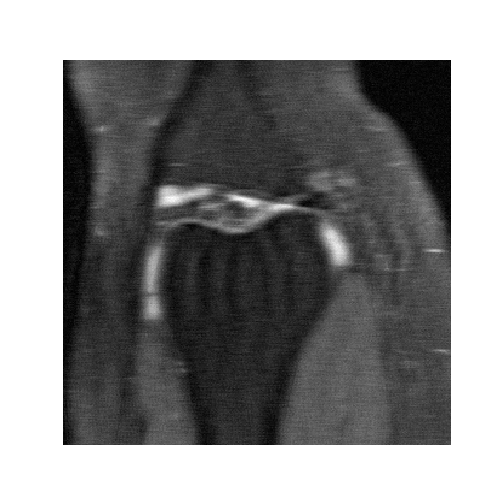
\includegraphics[width=0.4\textwidth]{Figures/dl_mri_figures/zfilled_recon_af4.png}};
            \node[below=-1em of knee] (knee_exp) {Aliased image};
            \draw[->, line width=0.3cm, color=DarkBlue] (kspace.east) -- ($(knee.west)+(0.8cm,0)$) node [below,midway, color=DarkBlue!87, yshift=-0.3cm] {\textbf{IFFT}};
        \end{tikzpicture}
    \end{center}

    \pause
    \textbf{Redundancy}, or \textbf{sparsity, symmetry, structure or a priori information}, is the key.
    
\end{frame}

\begin{frame}{Parallel imaging}
    % "forging" the redundancy
    % We can build more redundancy in the measuring system by using \textbf{more antennas (called coils)} to measure the magnetic signal.
    More redundancy using \textbf{more antennas (called coils)} $\Rightarrow$ \textbf{Parallel Imaging~(PI)}
    \begin{figure}
        \centering
        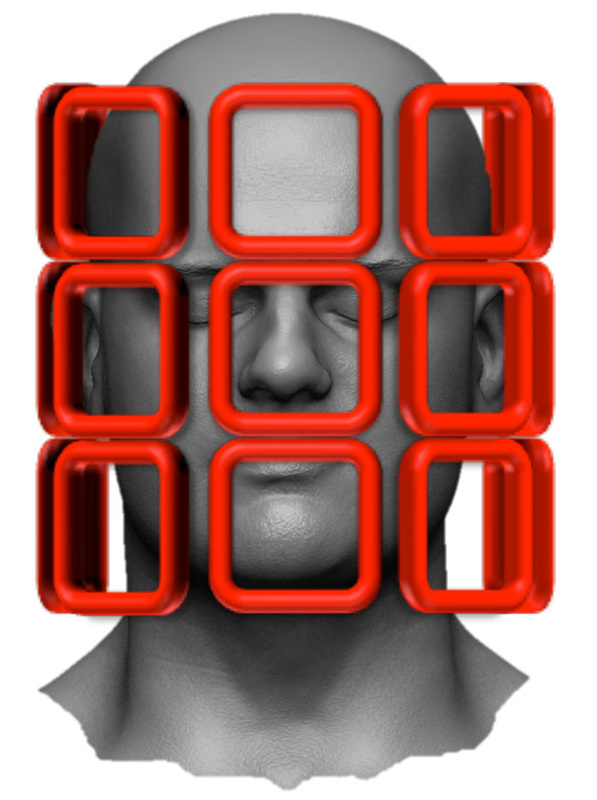
\includegraphics[height=0.4\textheight]{Figures/intro_figures/multicoil.jpg}
    \end{figure}
     
    % This technique is called \textbf{Parallel Imaging~(PI)}. 
    % A reconstruction algorithm is now needed to handle the multi-coil undersampled data.
        % \textbf{SENSE}\footfullcite{Pruessmann1999SENSE:MRI} and \textbf{GRAPPA}\footfullcite{Griswold2002GeneralizedGRAPPA} are such algorithms.    
    Multi-coil reconstruction algorithms: \textbf{SENSE}\footfullcite{Pruessmann1999SENSE:MRI} and \textbf{GRAPPA}\footfullcite{Griswold2002GeneralizedGRAPPA}.
    % GRAPPA + SENSE examples
\end{frame}

\begin{frame}{The example of GRAPPA}
    \begin{figure}
        \centering
        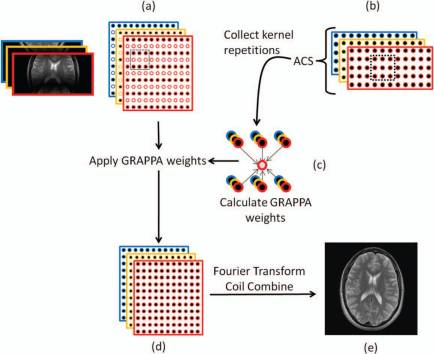
\includegraphics[height=0.6\textheight]{Figures/intro_figures/GRAPPA.jpeg}
        \caption{\label{fig:GRAPPA}\textbf{GRAPPA illustration.} Image courtesy of \citet{deshmane2012parallel}.
        }
    \end{figure} 
\end{frame}

\begin{frame}{Limits of Parallel Imaging}
    % Max AF
    Acceleration function of the number of coils.\\
    Resulting acceleration: 2 in 2D, 8 in 3D.
    % ow: https://www.siemens-healthineers.com/magnetic-resonance-imaging/options-and-upgrades/clinical-applications/syngo-grappa says 2,3
\end{frame}